\documentclass[document.tex]{subfiles}
\begin{document}
\section*{Exercise 1:}

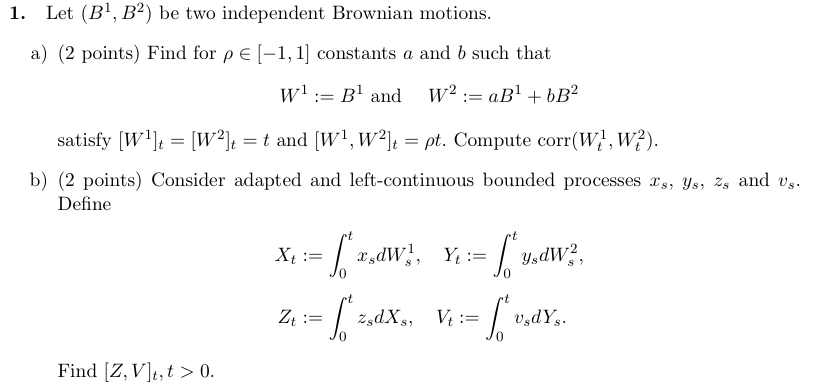
\includegraphics[width=\textwidth]{ex1.png}

\subsection*{a)}
\begin{align*}
	\rho t &= \qcVar{W^1}{W^2} \\
	&= \qcVar{B^1}{a B^1 + b B^2} \\
	&\text{, since the quadratic covariation is bilinear in it's arguments}\\
	&= a \qcVar{B^1}{B^1} + b \underbrace{\qcVar{B^1}{B^2}}_{=0, \text{since} B^1 \text{and} B^2 \text{independent}} \\
	&= a \qVar{B^1} \\
	&= a t \\
\Rightarrow a &= \rho	 
\end{align*}
\begin{align*}
	t &= \qVar{W^2} \\
	&= \qcVar{W^2}{W^2}\\
	&= \qcVar{a B^1 + b B^2}{a B^1 + b B^2}\\
	&= \qcVar{a B^1 + b B^2}{a B^1} + \qcVar{a B^1 + b B^2}{b B^2}\\
	&= \qcVar{aB^1}{aB^1} + \underbrace{\qcVar{bB^2}{aB^1}}_{=0} + \underbrace{\qcVar{aB^1}{bB^2}}_{=0} + \qcVar{bB^2}{bB^2}\\
	&= a^2 \underbrace{\qcVar{B^1}{B^1}}_{\qVar{B^1}=t}+ b^2 \underbrace{\qcVar{B^2}{B^2}}_{\qVar{B^2}=t} \\
\Rightarrow	b^2 &= 1 - a^2
\end{align*}


\end{document}
